

\tikzset{every picture/.style={line width=0.75pt}} %set default line width to 0.75pt        

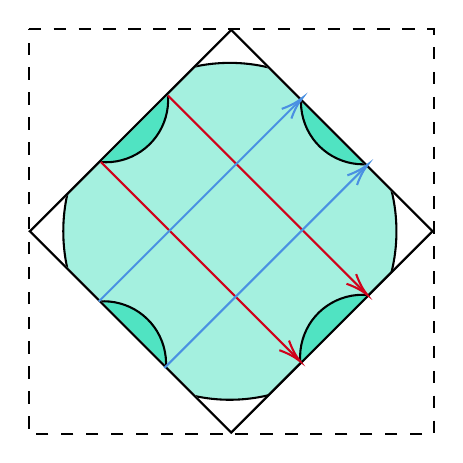
\begin{tikzpicture}[x=0.75pt,y=0.75pt,yscale=-1,xscale=1]
%uncomment if require: \path (0,300); %set diagram left start at 0, and has height of 300

%Shape: Path Data [id:dp28391475851762316] 
\draw  [fill={rgb, 255:red, 80; green, 227; blue, 194 }  ,fill opacity=0.52 ] (325.74,53.12) .. controls (332.21,53.12) and (338.5,53.9) .. (344.52,55.36) -- (403.58,114.41) .. controls (405.16,120.77) and (406,127.42) .. (406,134.28) .. controls (406,141.11) and (405.17,147.74) .. (403.6,154.07) -- (344.44,213.22) .. controls (338.44,214.67) and (332.18,215.44) .. (325.74,215.44) .. controls (319.93,215.44) and (314.25,214.81) .. (308.79,213.62) -- (247.46,152.3) .. controls (246.17,146.5) and (245.48,140.47) .. (245.48,134.28) .. controls (245.48,128.06) and (246.17,122) .. (247.48,116.19) -- (308.72,54.95) .. controls (314.2,53.75) and (319.9,53.12) .. (325.74,53.12) -- cycle ;
%Shape: Arc [id:dp4924996181571455] 
\draw  [draw opacity=0][fill={rgb, 255:red, 80; green, 227; blue, 194 }  ,fill opacity=1 ] (392.41,101.91) .. controls (378.45,103.05) and (365.16,94.24) .. (361.16,80.25) .. controls (360.17,76.79) and (359.83,73.29) .. (360.07,69.89) -- (390,72) -- cycle ; \draw   (392.41,101.91) .. controls (378.45,103.05) and (365.16,94.24) .. (361.16,80.25) .. controls (360.17,76.79) and (359.83,73.29) .. (360.07,69.89) ;
%Shape: Square [id:dp8258883831288684] 
\draw   (326.42,37.25) -- (423.42,134.25) -- (326.42,231.25) -- (229.42,134.25) -- cycle ;
%Shape: Arc [id:dp34996890506368183] 
\draw  [draw opacity=0][fill={rgb, 255:red, 80; green, 227; blue, 194 }  ,fill opacity=1 ] (263.59,100.91) .. controls (277.55,102.05) and (290.84,93.24) .. (294.84,79.25) .. controls (295.83,75.79) and (296.17,72.29) .. (295.93,68.89) -- (266,71) -- cycle ; \draw   (263.59,100.91) .. controls (277.55,102.05) and (290.84,93.24) .. (294.84,79.25) .. controls (295.83,75.79) and (296.17,72.29) .. (295.93,68.89) ;
%Shape: Arc [id:dp4561026088076878] 
\draw  [draw opacity=0][fill={rgb, 255:red, 80; green, 227; blue, 194 }  ,fill opacity=1 ] (392,164.96) .. controls (378.04,163.82) and (364.75,172.63) .. (360.75,186.61) .. controls (359.75,190.08) and (359.41,193.58) .. (359.65,196.97) -- (389.59,194.87) -- cycle ; \draw   (392,164.96) .. controls (378.04,163.82) and (364.75,172.63) .. (360.75,186.61) .. controls (359.75,190.08) and (359.41,193.58) .. (359.65,196.97) ;
%Shape: Arc [id:dp15892708580174042] 
\draw  [draw opacity=0][fill={rgb, 255:red, 80; green, 227; blue, 194 }  ,fill opacity=1 ] (262.59,168.09) .. controls (276.55,166.95) and (289.84,175.76) .. (293.84,189.75) .. controls (294.83,193.21) and (295.17,196.71) .. (294.93,200.11) -- (265,198) -- cycle ; \draw   (262.59,168.09) .. controls (276.55,166.95) and (289.84,175.76) .. (293.84,189.75) .. controls (294.83,193.21) and (295.17,196.71) .. (294.93,200.11) ;
%Shape: Right Triangle [id:dp9873621257073468] 
\draw  [color={rgb, 255:red, 255; green, 255; blue, 255 }  ,draw opacity=1 ][fill={rgb, 255:red, 255; green, 255; blue, 255 }  ,fill opacity=1 ] (229.42,134.25) -- (326.42,37.25) -- (229.42,37.25) -- cycle ;
%Shape: Right Triangle [id:dp20784307542005132] 
\draw  [color={rgb, 255:red, 255; green, 255; blue, 255 }  ,draw opacity=1 ][fill={rgb, 255:red, 255; green, 255; blue, 255 }  ,fill opacity=1 ] (423.42,134.25) -- (326.42,37.25) -- (423.42,37.25) -- cycle ;
%Shape: Right Triangle [id:dp19958209753051315] 
\draw  [color={rgb, 255:red, 255; green, 255; blue, 255 }  ,draw opacity=1 ][fill={rgb, 255:red, 255; green, 255; blue, 255 }  ,fill opacity=1 ] (424,134.83) -- (327,231.83) -- (424,231.83) -- cycle ;
%Shape: Right Triangle [id:dp13150240831757665] 
\draw  [color={rgb, 255:red, 255; green, 255; blue, 255 }  ,draw opacity=1 ][fill={rgb, 255:red, 255; green, 255; blue, 255 }  ,fill opacity=1 ] (230,134.83) -- (327,231.83) -- (230,231.83) -- cycle ;
%Shape: Square [id:dp6591394813744926] 
\draw   (326.42,37.25) -- (423.42,134.25) -- (326.42,231.25) -- (229.42,134.25) -- cycle ;
%Shape: Square [id:dp30244562238327477] 
\draw  [dash pattern={on 4.5pt off 4.5pt}] (228.83,36.67) -- (424,36.67) -- (424,231.83) -- (228.83,231.83) -- cycle ;
%Straight Lines [id:da43761852194250594] 
\draw [color={rgb, 255:red, 208; green, 2; blue, 27 }  ,draw opacity=1 ]   (295.93,68.89) -- (390.59,163.54) ;
\draw [shift={(392,164.96)}, rotate = 225] [color={rgb, 255:red, 208; green, 2; blue, 27 }  ,draw opacity=1 ][line width=0.75]    (10.93,-3.29) .. controls (6.95,-1.4) and (3.31,-0.3) .. (0,0) .. controls (3.31,0.3) and (6.95,1.4) .. (10.93,3.29)   ;
%Straight Lines [id:da018143618520460425] 
\draw [color={rgb, 255:red, 208; green, 2; blue, 27 }  ,draw opacity=1 ]   (263.59,100.91) -- (358.24,195.56) ;
\draw [shift={(359.65,196.97)}, rotate = 225] [color={rgb, 255:red, 208; green, 2; blue, 27 }  ,draw opacity=1 ][line width=0.75]    (10.93,-3.29) .. controls (6.95,-1.4) and (3.31,-0.3) .. (0,0) .. controls (3.31,0.3) and (6.95,1.4) .. (10.93,3.29)   ;
%Straight Lines [id:da48286677460832284] 
\draw [color={rgb, 255:red, 74; green, 144; blue, 226 }  ,draw opacity=1 ]   (262.59,168.09) -- (359.37,71.31) ;
\draw [shift={(360.79,69.89)}, rotate = 495] [color={rgb, 255:red, 74; green, 144; blue, 226 }  ,draw opacity=1 ][line width=0.75]    (10.93,-3.29) .. controls (6.95,-1.4) and (3.31,-0.3) .. (0,0) .. controls (3.31,0.3) and (6.95,1.4) .. (10.93,3.29)   ;
%Straight Lines [id:da3902094286940192] 
\draw [color={rgb, 255:red, 74; green, 144; blue, 226 }  ,draw opacity=1 ]   (294.21,200.11) -- (391,103.32) ;
\draw [shift={(392.41,101.91)}, rotate = 495] [color={rgb, 255:red, 74; green, 144; blue, 226 }  ,draw opacity=1 ][line width=0.75]    (10.93,-3.29) .. controls (6.95,-1.4) and (3.31,-0.3) .. (0,0) .. controls (3.31,0.3) and (6.95,1.4) .. (10.93,3.29)   ;




\end{tikzpicture}